\documentclass[10pt,twocolumn,letterpaper]{article}
%% Language and font encodings
\usepackage[english]{babel}
\usepackage[utf8x]{inputenc}
\usepackage[T1]{fontenc}
% xcolor is the package between braces and between brackets is the option that we want to use
\usepackage{fancyhdr}
\usepackage{biblatex}
\usepackage{array}
\usepackage[color]{showkeys}
\usepackage{etoolbox}
\usepackage{graphicx,tabularx}
\usepackage{amsfonts} 
%% Sets page size and margins
\usepackage[a4paper,top=3cm,bottom=2cm,left=3cm,right=3cm,marginparwidth=1.75cm]{geometry}
%% Useful packages
\usepackage{amsmath}
\usepackage[colorlinks=true, allcolors=blue]{hyperref}
\fancypagestyle{plain}{%
  \fancyhead{}
  \fancyfoot{}
  \fancyfoot[R]{\thepage}
  \fancyfoot[L]{[INFOMR] Multimedia Retrieval - Utrecht University}
}
\pagestyle{plain}
\title{%
  3D Mesh Retrieval System \\
  \large Multimedia Retrieval \\
    Utrecht University}
    
\author{
  Da Costa Barros, Fabien [0720823]\\
  \url{f.n.dacostabarros@uu.students.nl}
  \and
  Bagheri, Soheil [6208908]\\
  \url{s.bagheri@students.uu.nl}
}
\date{\today}
\addbibresource{refs.bib}                                                                     
\begin{document}
\maketitle
\selectlanguage{english}
\section*{Introduction}
With the advance in modeling software and 3D scanners, the speed of 3D content creation increased rapidly. Nowadays, much 3D content has been produced, and people are still creating many more objects constantly. These kinds of contents are usually stored in so-called shape databases. But, there is a challenge to browse and find the 3D objects of interest within these numerous amounts of data.\\ \\
Several techniques have already been presented for finding desired data in these shape databases. For example, searching by keyword, browsing the database along a few predefined categories, or content-based shape retrieval (CBSR). Although the first two options do not need a sample model for searching in a database, they need more effort to label or categorize these contents. On the other hand, there is content-based shape retrieval which can retrieve all the similar samples to the existing query shape.\\ \\
In this project, we want to categorize the 3D objects of a database based on their shape similarity. This process will be done by normalizing all the objects and extracting some general features from them. Then, we can divide similar objects based on their similarity in their features. Also, there would be a content-based shape retrieval that can find similar 3D objects based on the feature extracted from the given query shape and compared to other objects in the database.

\section{Selection and setup the work environment}
In this section, four different related packages have been tested and compared. The Comparison of these packages has been done based on several features that might be useful in the future sections of this project. For example, being able to re-mesh objects, scaling them, rotating them, and moving them are the feature that can be useful in the process of normalizing the 3d objects in the database. Also, having some information about the 3d objects, like the number of vertices and faces, is necessary for understanding if these 3d objects are normalized or not. On the other hand, this package must support different formats that are usually used to store 3d objects.
In this case, we narrowed down the packages that work with Python language and well-known between the community. So, we tested and analyzed "Pymesh", "PyMeshLab", "TriMesh", and "Open3D". Results can be found in the table 1.\\ \\
We wanted to be able to open "PLY", "OFF", "OBJ", and "STL" formats. "PLY" and "OFF" formats were discussed in the lecture, while "OBJ" and "STL" are really common. All of them were able to open "PLY", "OFF", "OBJ", and "STL" formats, so that was not really discriminating. \\ \\
	We tried to compare the different re-meshing, repairing and extraction features with our current knowledge and thought that PyMeshLab and Open3D seems to be quite good. The complexity was also one of our requirements as from previous experience less complex library offers less options. \\ \\
	After achieving step 1 with four of those libraries, we try to find a balance between number of dependencies, options proposed for visualizing and analysis. Then we decide to choose "PyMeshLab"\cite{pymeshlab}
Our project has three main dependencies. "PyMeshLab", "Polyscope", and "Numpy", and it runs with Python 3.9. \\ 
\begin{table*}[ht]
    	\hspace*{-0.1\linewidth}\begin{tabular}{|p{0.25\linewidth}|p{0.2\linewidth}|>{\centering}p{0.15\linewidth}|>{\centering}p{0.15\linewidth}|>{\centering}p{0.15\linewidth}|>{\centering\arraybackslash}p{0.15\linewidth}|}
    		\hline
     		Features category & Desired Fetures & PyMesh & PyMeshLab & TriMesh & Open3D \\ \hline
    	    3D format supported & PLY & X & X & X & X \\
    	    ~ & OFF & X & X & X & X \\
    	    ~ & OBJ & X & X & X & X \\
    	    ~ & STL & X & X & X & X \\ \hline
    	    Repairing & Isolated Vertices & X & X & X & To implement \\ 
     		~ & Duplicated Vertices & X & X & X & To implement \\ 
    	    ~ & Duplicated Faces & X & X & X & To implement \\ \hline
    	    Remeshing & Uniform sampling & X & X & X & X \\ \hline
    	    Analysis features & ~ & Simple & Rich & Sufficient & Rich \\ \hline
    	    Visualisation features & Scale & 0 & X & X & X \\ 
   		    ~ & Pan & 0 & X & X & X \\ 
     		~ & Rotate & 0 & X & X & X \\
        	~ & Screenshot & 0 & X & 0 & X \\ 
        	~ & Multiple mesh & 0 & X & 0 & X \\ \hline
        	Language & Source code & 70\% C++ \newline 20\% Python \newline 10\% C  & 80\% C++ \newline 20\%Python & 100\% Python & 80\% C++ \newline 10\% Python \newline 10\% Cuda \\ \hline
        	Number of dependencies & ~ & 7 & 2 & 3 & 0 \\ \hline
        	Interface of preview windows & ~ & None & Advanced & Minimalistic &~ \\ \hline
        	Visualisation interface & Shading methods & None & Flat & Flat & Flat \\ \hline
        	Installation tools & Pip or Anaconda & Docker & Pip & Pip & Pip \\ \hline
    	\end{tabular}
    	 \caption{In-built features for different Python libraries}
  		\label{tab:libraries}
	\end{table*} \\ \\


\section{Rendering}
We have two scripts for this step called "main.py" and "render.py" Where "main.py" verifies the console arguments and calls the render function from "render.py". The first argument passed through is the path of the file. \\ \\
In "render.py", there is a function called "render". This function loads the mesh and displays the vertices and the mesh of the 3D object. PyMeshLab has a built-in function ".show\_polyscope" that shows a mesh. While we found it more interesting to override it with polyscope functions to have more control if we need to upgrade anything. The result of the mesh visualization script can be found in Figure \ref{fig:ant-mesh}. The 3D mesh visualization windows offered many functionalities.

	
	
\begin{figure}[h!]
\begin{center}
  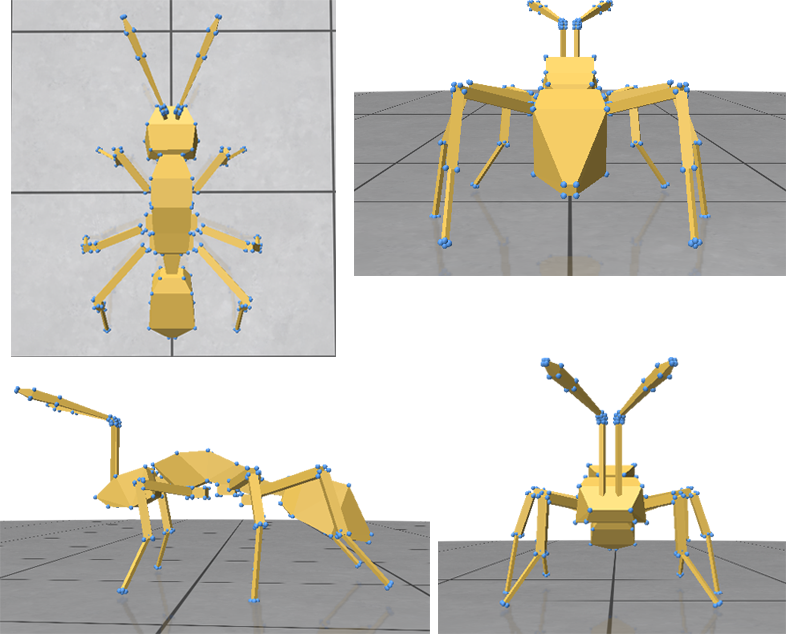
\includegraphics[width=0.5\textwidth]{ant}
  \caption{Visualisation of an ant mesh}
  \label{fig:ant-mesh}
  \end{center}
\end{figure}
%\section*{Acknowledgements}
%Anyone to thank/credit for helping your team along the way? This is the place to do it.
\medskip
\printbibliography
\end{document}